% v1.0 released 28th January 1994

%\documentclass[a4paper, 12pt, usenatbib]{article}
\documentclass[a4paper, 11pt, usenatbib]{article}
\usepackage[margin=0.8in, top = 1.2in, bottom=1.4in]{geometry}
\usepackage[fleqn]{amsmath}
\usepackage{ragged2e}
\usepackage{graphicx}
%\usepackage[skip=0pt]{caption}
\usepackage{caption}
\usepackage{url}
\usepackage{amssymb}
\usepackage{framed}


\usepackage{enumitem}
\usepackage{float}
\usepackage{wrapfig}
\restylefloat{figure}
\setlist[itemize]{  
  listindent= 4em,
%  parsep=0pt,
}
\setlength{\parindent}{0mm}
\setlength{\parskip}{1em}
\setitemize[0]{leftmargin=10pt,itemindent=12pt}
\usepackage{fancyhdr}

%\pagestyle{fancy}
%\fancyhf{}

\setlength\headheight{24pt} 

\usepackage{color}
\newcommand{\myitem}{$\text{}\qquad\bullet\ $}
\newcommand{\mynumber}{$\text{}\qquad\ $}


\begin{document}

\title{Stock Price Forecasting Modelling}
\author{Chuanwu (Charles) Liu}

\maketitle



\section{Features}
This task is a time series forecasting problem. Considering the significant data volume, I decide to use recurrent neural networks to solve this task. At time $t$, the input features are selected as the open, high, low and close prices and the trading volume at past times $t-N$, $t-N+1$, $\cdots$, $t-1$, $t$, where $N$ is the lookback time. The volume is included, because it reflects the market's reaction to the prices and provides additional information. The derived features such as high/low are not included, because a neural network is able to approach these.
Depending on the target feature, two models are considered:
\begin{enumerate}
\item The regression model, in which the target value is the close price at $t+1$, represented as $P_{t+1}^c$.

\item The classification model, in which the future close return $r_{t, t+1} = P_{t+1}^c / P_t - 1$ is calculated and the binary classification target is 1 if $r_{t, t+1}$ is positive or 0 if else. 
\end{enumerate}

\section{Data Preprocessing}
\subsection{Time series}
All valid trading dates are considered as consecutive dates. Non-trading dates including weekends and public holidays are ignored. Some tickers appear after Jan 2015, the dates before their first appearance is also ignored.

\subsection{Missing values}
For a selected ticker, if a data point is not found on a trading date after its first appearance, it is defined as a missing value. There are a number of methods have been considered for the handling missing values:
\begin{enumerate}


\item Discard samples with missing samples. This is the simplest way and and it does not introduce bias from missing value handling methods. However, in time series forecasting, the data removal will break the time consecutiveness.

\item Impute missing values with a value that has its meaning and distinct from all other values such as 0. This is acceptable, as neural networks will learn from the data that the value 0 means missing data and will start ignoring the value. However if missing value is included in the test set, we have to make sure the missing values are also included in the training set.

\item Impute missing values with the mean or median of each feature. Such a constant has small contribution to the loss function. However, it introduces bias if most of existing values are far from the mean or median.

\item Impute missing values with other predictive models such as linear interpolation, moving average, AIMA and Exponential Smoothing. However, this method requires extra effort to build predictive models for error handling. Subject to the model, the artificial patterns from the missing value handling model model may mislead the neural networks.
 
\end{enumerate}

In my Jupyter notebook, four methods are implemented: (i) Remove missing values; (ii) Replace missing values with 0; (iii) Replace missing values with column means; and (iv) Linear interpolation. Their performances vary from ticker to ticker depending on the pattern of the signal and number of missing values. However, in this note, too reduce the number of free parameter, only the tickers with no or few missing values such as ANZ, CBA, NAB and BHP are presented.


\subsection{Data Scaling}
The price columns and the volume column have different scales so that data scaling is needed. There are two commonly used data scaling methods: the standard scaling and the MinMax scaling. The MinMax scaling is adopted in this task. In contrast, the standard scaling will result negative prices and volumes. The MinMax scaling is defined as
\begin{equation}
X_\mathrm{norm} = \frac{X-X_\mathrm{min}}{X_\mathrm{max} - X_\mathrm{min}}
\end{equation}


\section{Close Price Regression}
In this model I use the prices and volumes of past days, e.g. the past five days to predict the close price of the next day.

\subsection{Error metric}
We need an error metric to measure the difference between the model prediction and the test data. Because our error corresponds to the gain or loss of currency which is measured in liner scale. The Mean Absolute Error (MAE) is used as the error metric. MAE is defined as
\begin{equation}
\mathrm{MAE} = \frac{\sum_{i=1}^n |y_\mathrm{pred} - y_\mathrm{real}|}{n},
\end{equation}
where $y_\mathrm{pred}$ and $y_\mathrm{real}$ are the predicted value and the real value respectively.

\subsection{Baseline model}
To evaluate of power of my model, I first build a simple model as the baseline. We expect our neural networks are able to overtake the simple model. In this simple model, I assume the close price remains same on the next day, i.e. $P_{t+1}^c$ = $P_{t}^c$.

\subsection{Recurrent Neural Networks}
Recurrent Neural Network (RNN) is one the powerful tools for modelling sequential data including time series data. A Long Short-Term Memory (LSTM) network, which is a type of RNN is implement for this time series forecasting problem. The structure of my neural network contains:
\begin{enumerate}
\item Four LSTM layers.
\item Four Dropout layers with drop out rate 0.2
\item One Dense layer with activation function relu
\item One Dense layer without activation
\end{enumerate}

The model is optimised with Adam optimizer. The loss function of the optimisation is MAE.

\subsection{Training, validation and test samples}
The data set is divided into training set (60\%), validation set (20\%) and test set (20\%). The validation set is for the parameter tuning and test set is for the evaluation of model performance.


\subsection{Hyper-Parameters}
There are a number of hyper-parameters in this model:
\begin{itemize}

\item Lookback time, which is the number of past days that is used as input.
\item Number of units in each layer. This is the dimension of the representation space (weight matrix) of each layer.
\item Number of iteration epochs. One epoch represents a full iteration over all the training data.
\end{itemize}
I have completed a number of runs to tune the hyper-parameters.
For example, to find out the number of iteration epochs.
I have plotted the loss function for training and validation set as shown in Figure \ref{fig:regression_epochs}. We can see  the model stop improving after $\sim 100$ epochs. Therefore 100 is adopted for epochs.

\begin{figure}
	\centering
	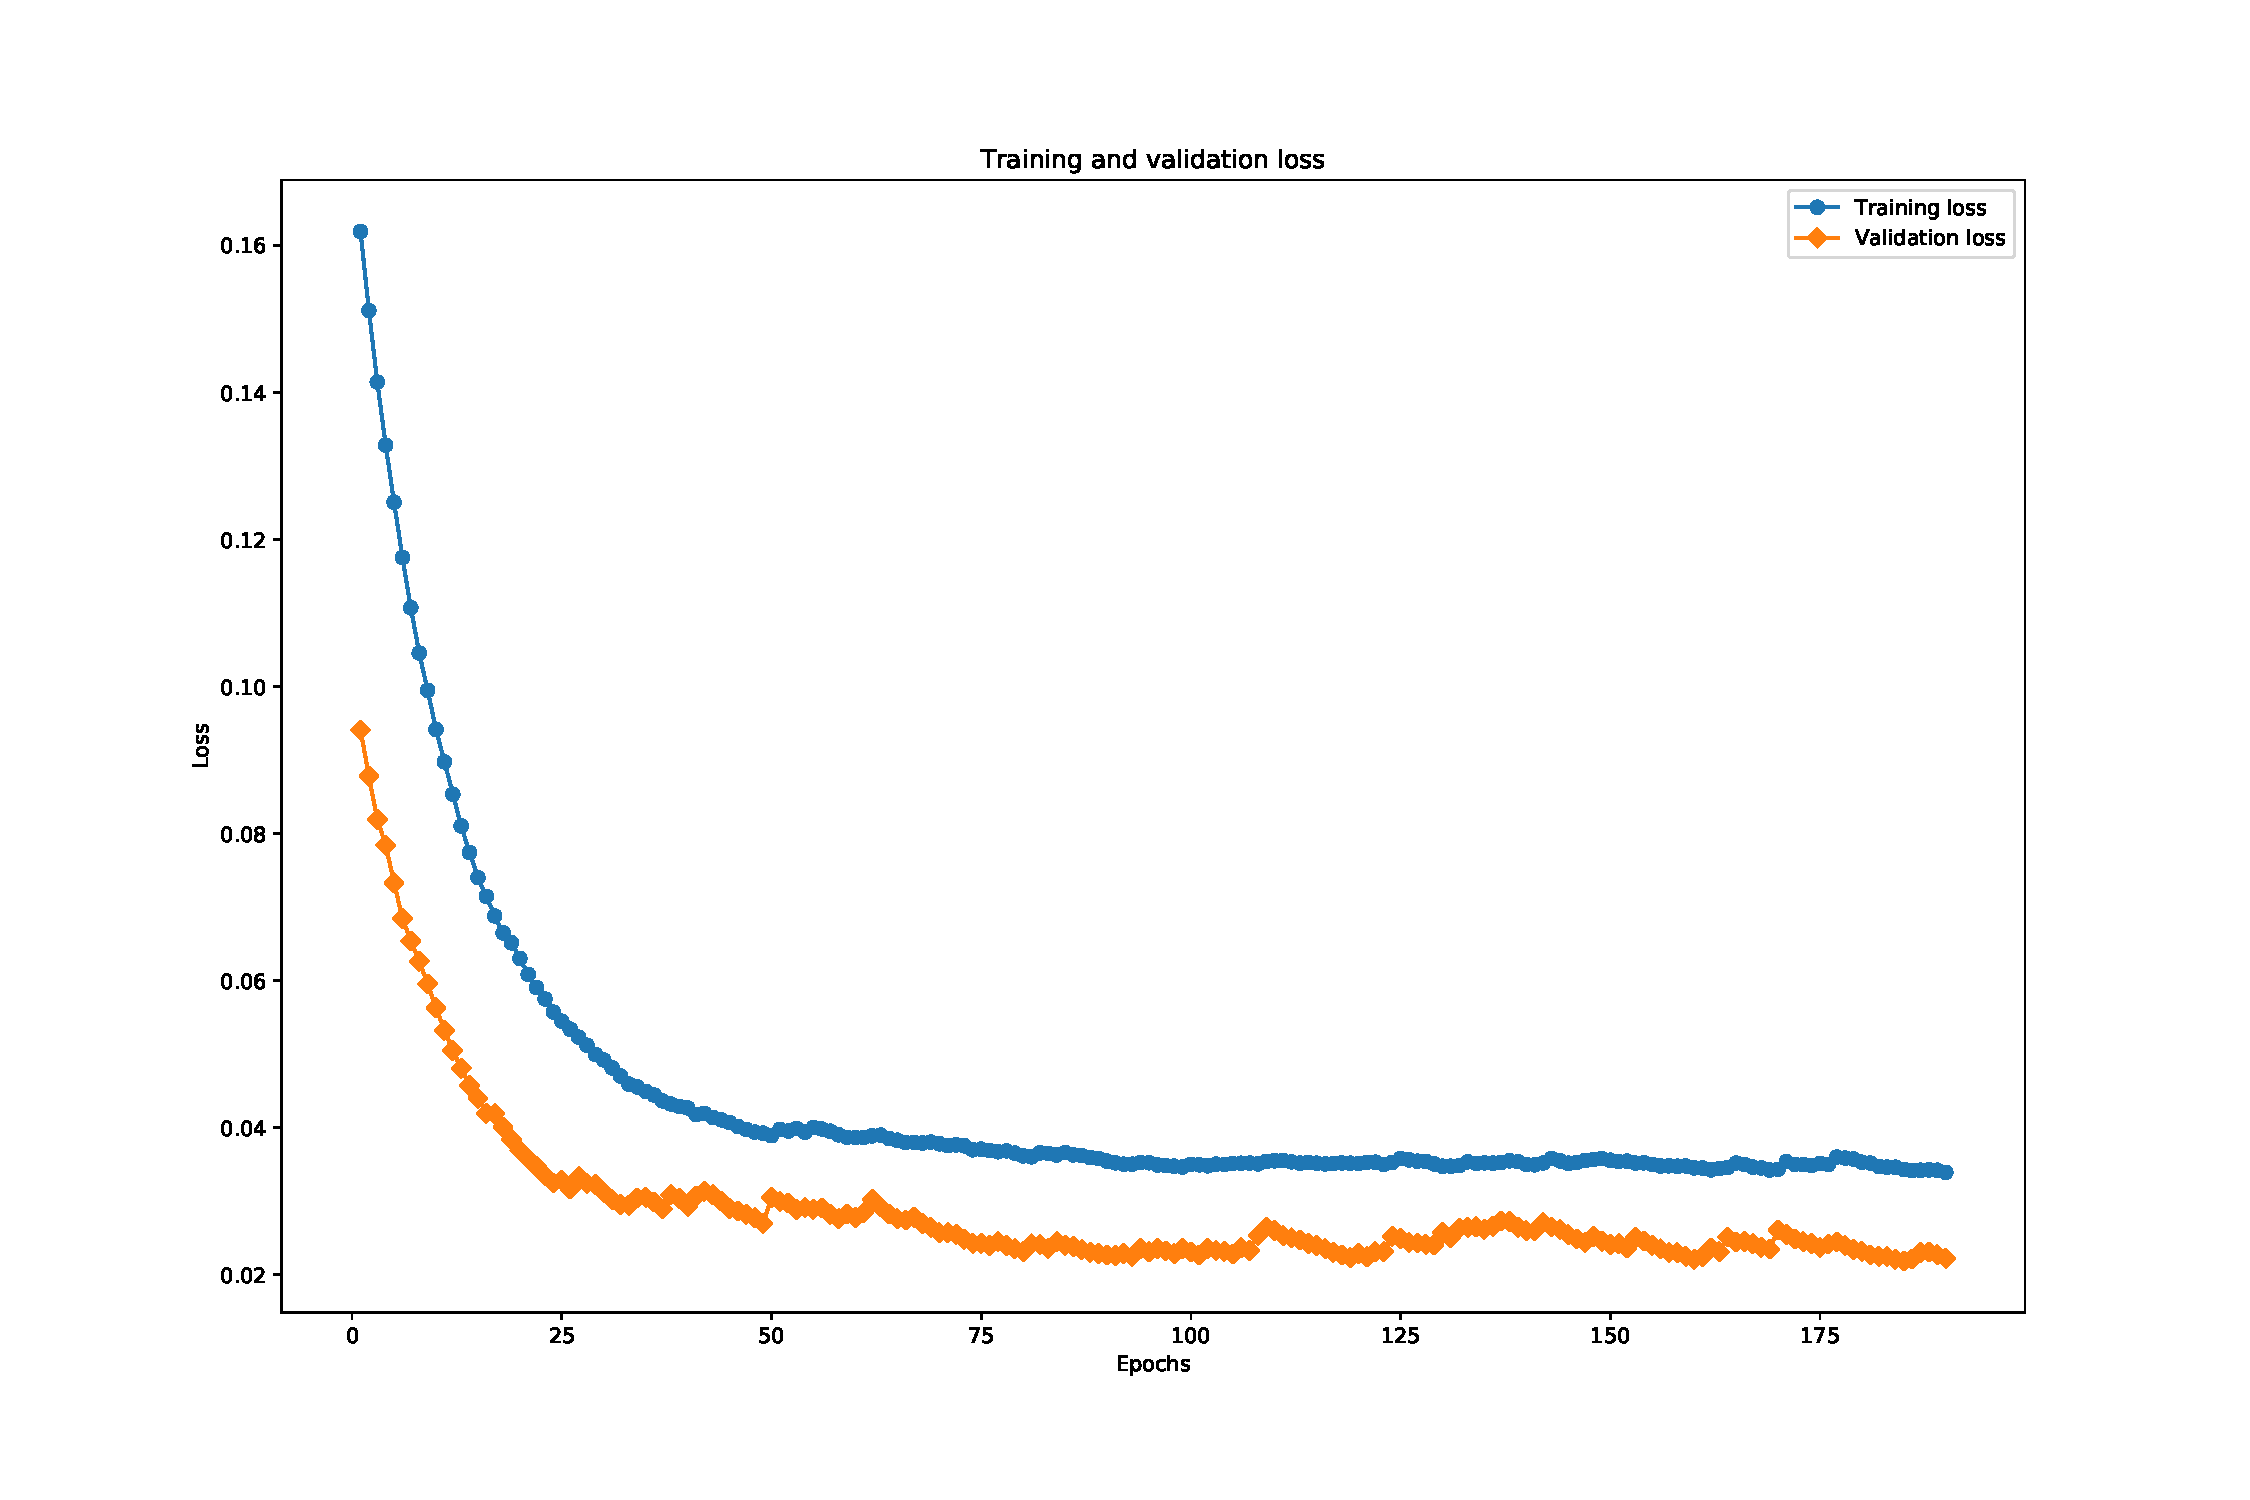
\includegraphics[width=0.9\textwidth]{./figures/regression_epochs.pdf}
	\caption[]
	{Loss of training and evaluation of 200 epochs for ANZ}
		\label{fig:regression_epochs}
\end{figure}

Based on the quick parameters turning for a couple of example tickers. The adopted parameter set in this work is
\begin{align*}
&\mathrm{Lookback\ time} = 5 \\
&\mathrm{Units\ of\ layers} = 64 \\
&\mathrm{Iteration\ epochs} = 100 
\end{align*}
However, the parameter tuning is a time consuming work and is essential for a neural network. Comprehensive investigations are required for tuning the model.

\subsection{Overfitting}
I have added one dropout layer after each LSTM layer to avoid the overfitting. That is why we don't see overfitting in Figure \ref{fig:regression_epochs}. 

\subsection{Results}

Figure \ref{fig:regression_test} shows the results of model prediction compared with the test samples. We see the model does not perform well.
This is because the model is not fully tuned. 
\begin{figure}
	\centering
	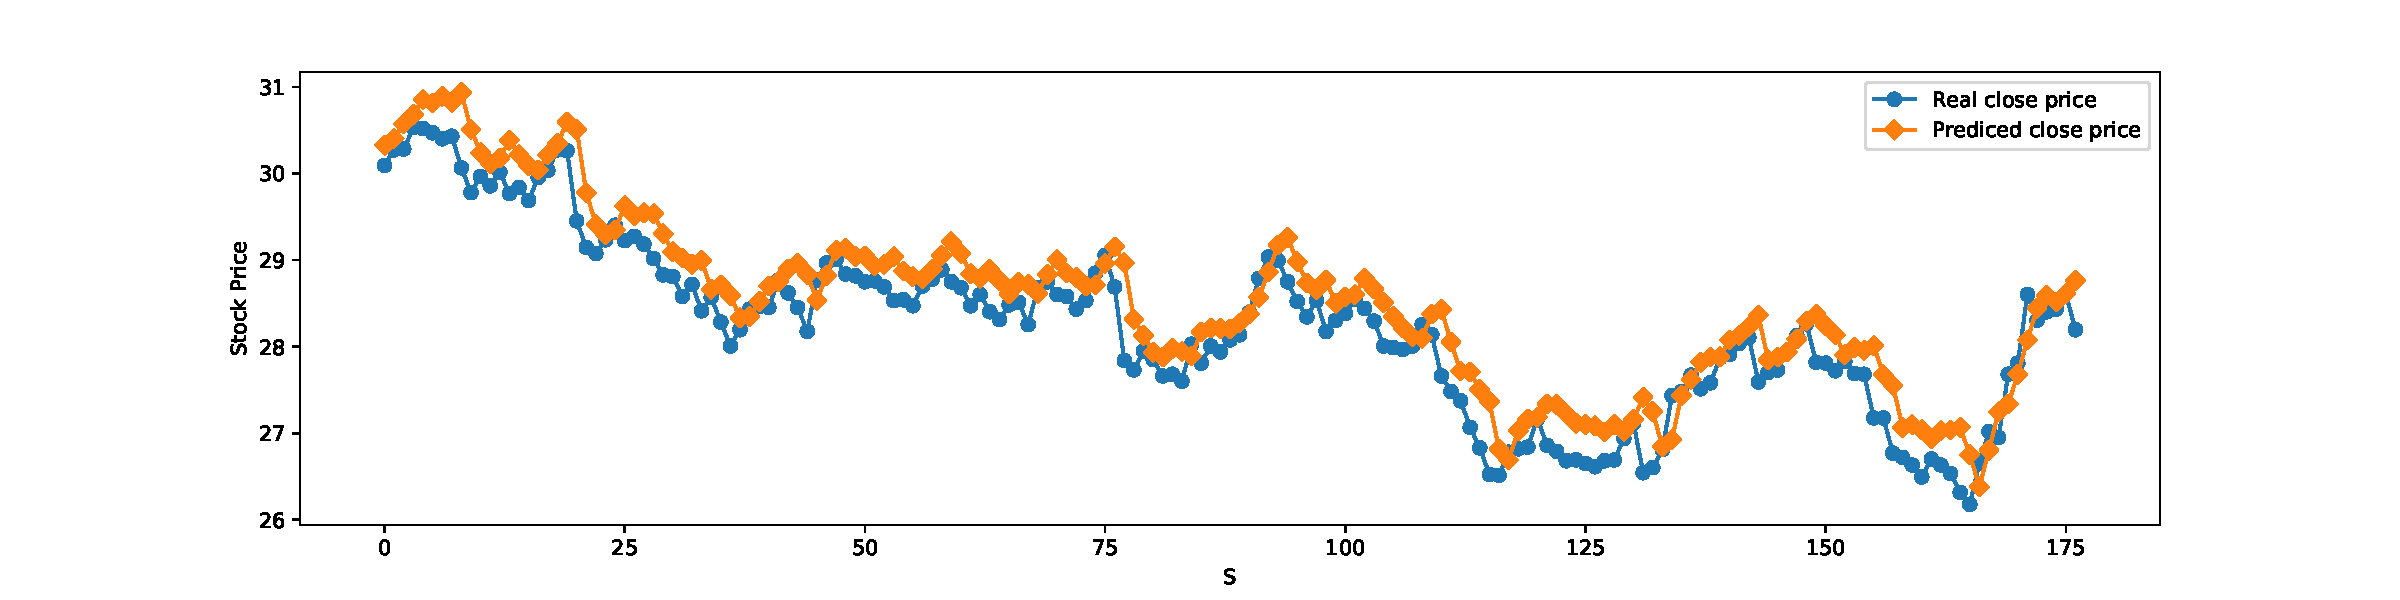
\includegraphics[width=0.9\textwidth]{./figures/regression_test.pdf}
	\caption[]
	{Loss of training and validation over 200 epochs for ANZ}
		\label{fig:regression_test}
\end{figure}

\begin{table}
 \caption{MAE loss of the regression}
 \label{tab:regression_loss}
 \centering
 \begin{tabular}
 { l  c  c  l }
  \hline
 Ticker & Baseline loss & Model loss\\
 \hline
 ANZ & 0.012 & 0.24 \\
 CBA & 0.018 & 0.76 \\
 NAB & 0.012 & 0.54\\
 BHP & 0.012 & 0.54 &\\

  \hline
 \end{tabular}
\end{table}  



\section{Binary Classification of future close return}
In this approach, I first calculate the future close return  $r_{t, t+1} = P_{t+1}^c / P_t - 1$ and the binary classification target is defined as
\begin{align*}
 1\ \mathrm{if} \ r_{t, t+1} > 0\\
 0\ \mathrm{if}\ r_{t, t+1} \le 0
\end{align*}

\subsection{Error metric}
The accuracy is adopted as the error metric. The accuracy is defined as
\begin{equation}
\mathrm{Accuracy} = \frac{\mathrm{Number\ of\ True\ Positive\ Predictions} + \mathrm{Number\ of\ True\ Nagative\ Predictions}} {\mathrm{Number\ of\ predictions}}
\end{equation}

\subsection{Baseline model}
The baseline model for the binary classification is that I assume the future close return has the same sign as close return, i.e. $\mathrm{sign}( r_{t, t+1})  = \mathrm{sign}(r_{t-1, t}) $.\\

\subsection{The Model}
The implemented network for this problem contains:
\begin{enumerate}
\item Two LSTM layers.
\item Two Dropout layers with drop out rate 0.2
\item One Dense layer with sigmoid activation. The sigmoid activation is use to convert numeric values to probability.
\end{enumerate}

The model is optimised with Adam optimizer. The loss function of the model is the binary crossentropy.

\subsection{Hyper Parameters}
The same set of hype parameters is adopted in this classification model. Figure	\label{fig:classification_epochs} shows the classification accuracy over 200 iteration epochs. We see that the accuracy reaches it maximum at $\sim 100$ and stop improving after that.
\begin{figure}
	\centering
	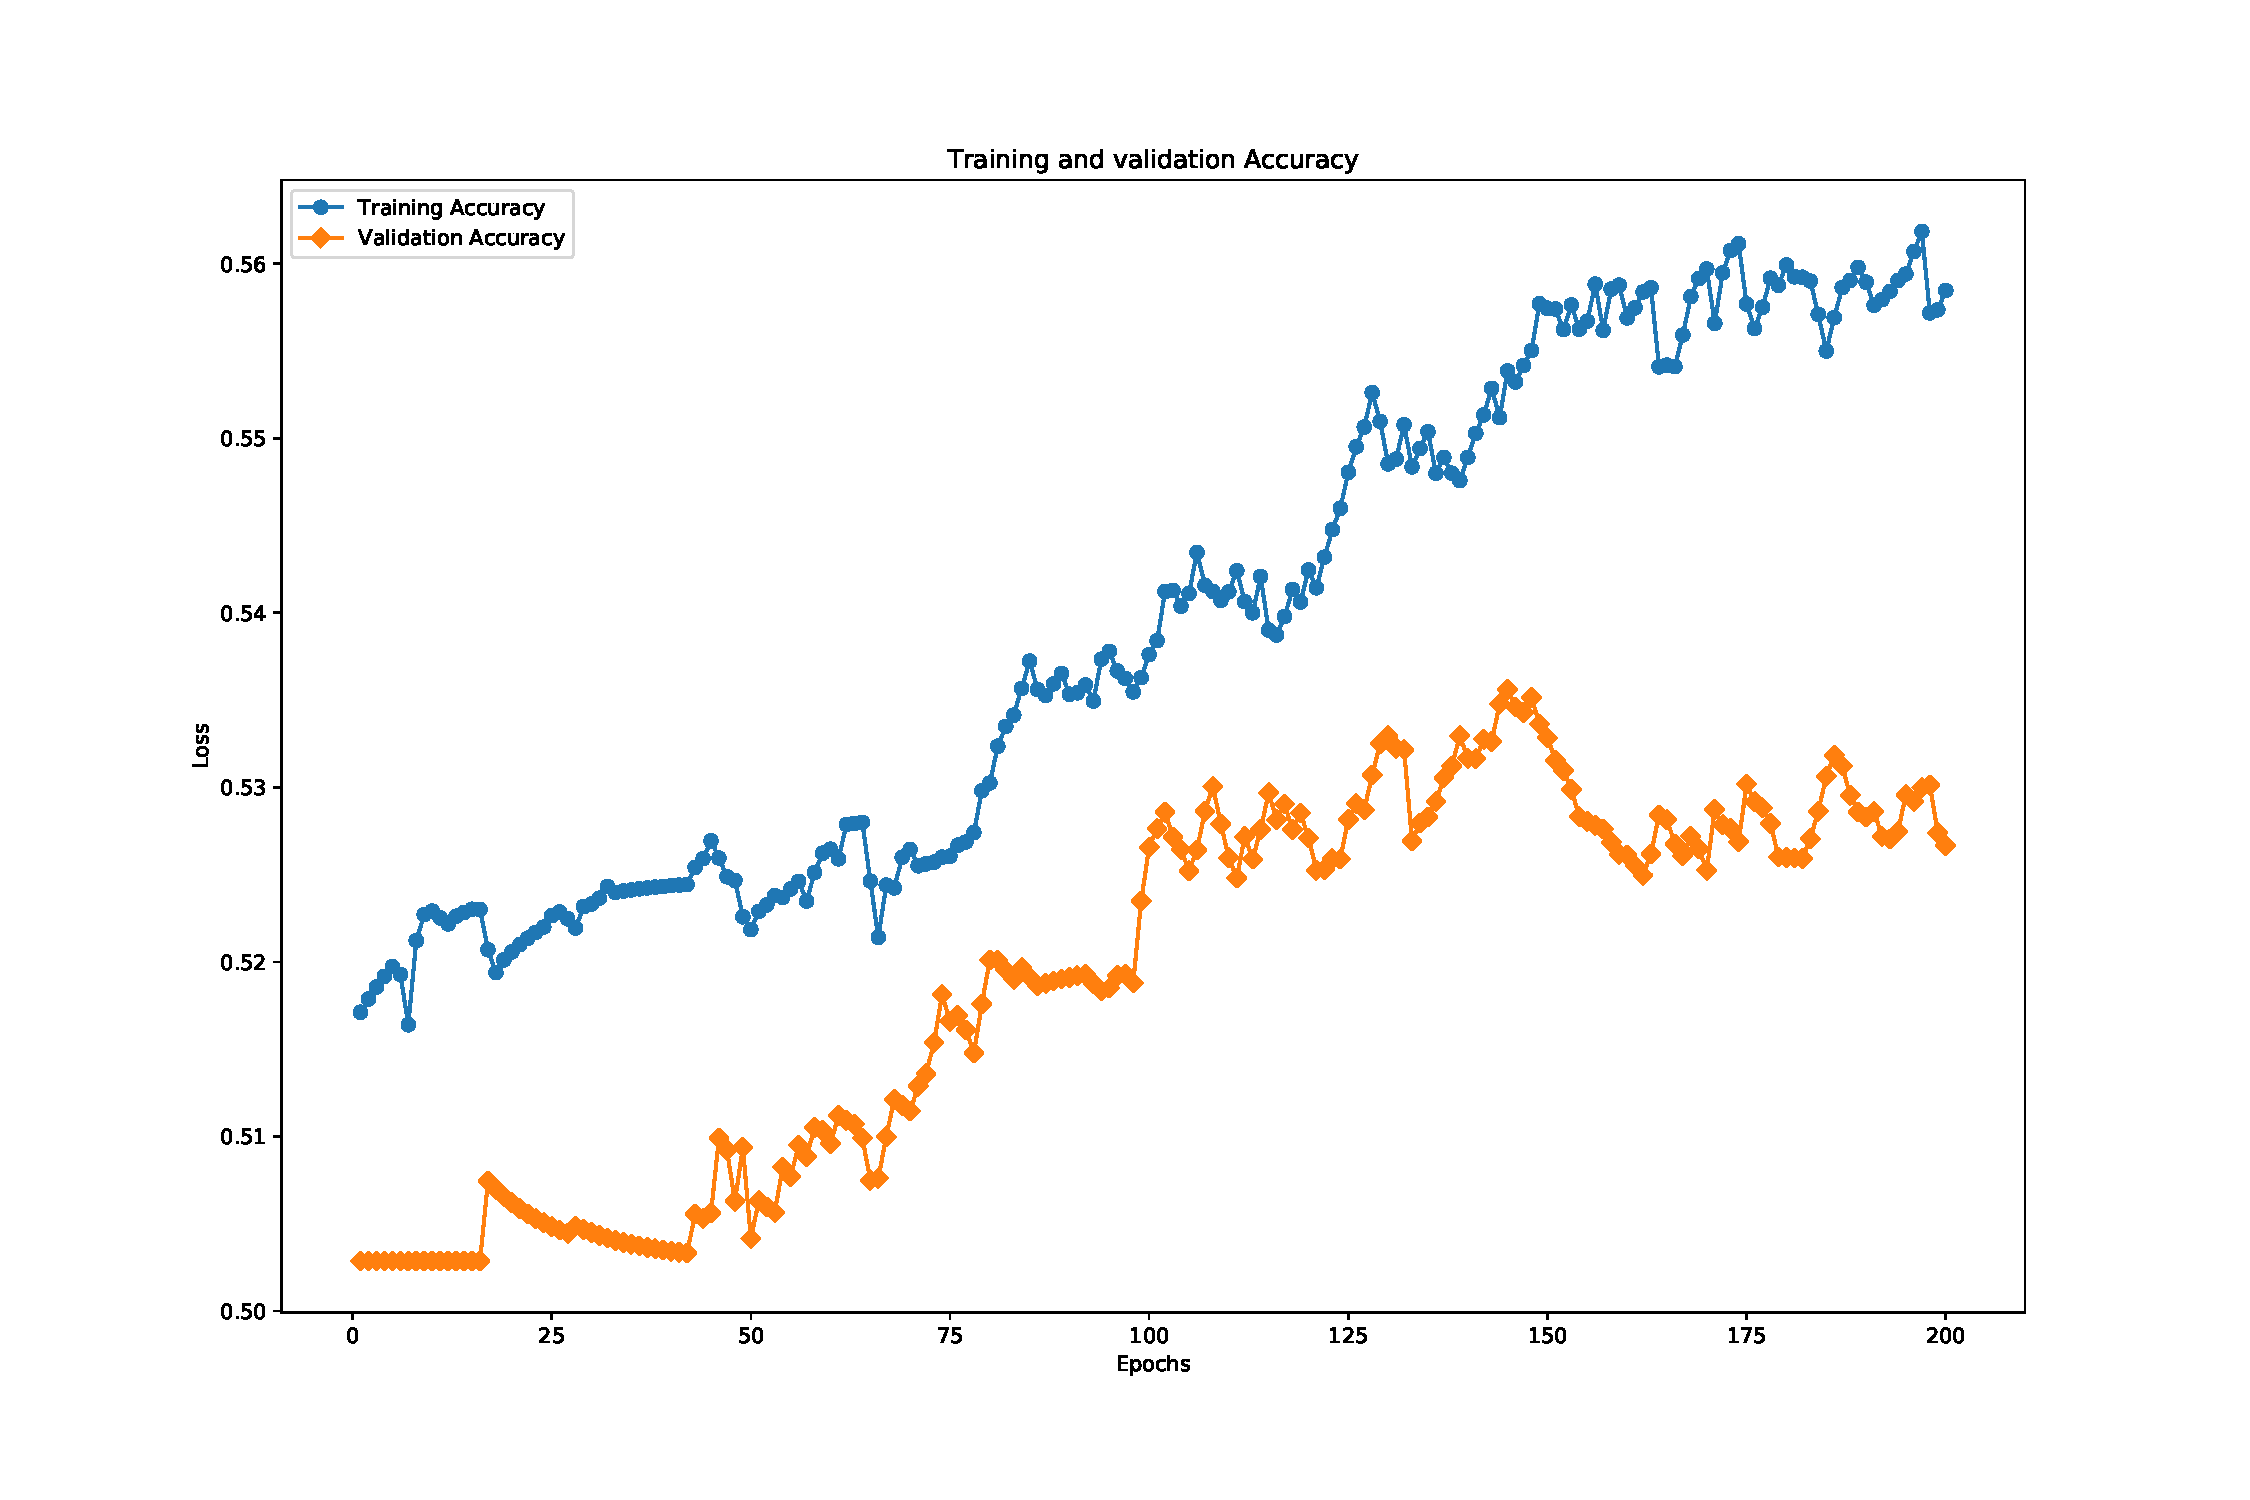
\includegraphics[width=0.9\textwidth]{./figures/classification_epochs.pdf}
	\caption[]
	{Classification accuracy of training and validation of 200 epochs for ANZ}
		\label{fig:classification_epochs}
\end{figure}

\subsection{Results}
The binary classification accuracy of example tickers is shown in Figure \ref{tab:classification_accuracy}. We see that this current classification model is not able to predict the future close return, except for NAB, which has a 
\begin{table}
 \caption{Accuracy of the binary classification}
 \label{tab:classification_accuracy}
 \centering
 \begin{tabular}
 { l  c  c  l }
  \hline
 Ticker & Baseline accuracy & Model accuracy\\
 \hline
 ANZ & 48\% & 46\% \\
 CBA & 45\% & 46\% \\
 NAB & 44\% & 54\%\\
 BHP & 57\% & 43\% &\\

  \hline
 \end{tabular}
\end{table}  

\section{Conclusion and Discussion}
We see in both regression and classification approach, the RNN model does not overtake the simple baseline. This may be because of two reasons:
\begin{enumerate}
 \item The models have not been well constructed and tuned. More comprehensive parameter tuning is required.
 \item The stock prices of the past is not a good indicator of future prices.
\end{enumerate}


\end{document}
